%----------------------------------------
%	Definitions
%----------------------------------------
\newcounter{problem}
\newcounter{solution}

\newenvironment{flattened}{
  \setlength{\parindent}{0cm}
}{}

\newcommand\Challenge{%
  \stepcounter{problem}%
  \textbf{Challenge \theproblem.}~%
  \setcounter{solution}{0}%
}
\newcommand\TheSolution{%
  \textbf{Solution:}\\%
}
\newcommand\ASolution{%
  \stepcounter{solution}%
  \textbf{Solution \thesolution:}\\%
}

\subsection{Challenges and refinements}
We are required to create deployment scripts using Ansible by which we can deploy our entire application on UniMelb Research Cloud. We faced several challenges while developing these roles and packages due to the cloud complexity and scenario requirements.

\begin{flattened}

\Challenge Mapping different volume and security group configuration with their respective VM instances

\TheSolution In order to solve this issue, we maintained volume and security group configuration mappings using \texttt{sds-infra-vars.yaml} file in sds-infra Ansible package. Using this mapping, we have implemented looping mechanism which creates new dictionary structure which can be then be used with \texttt{os\_server}.

\begin{figure}[H]
    \centering
    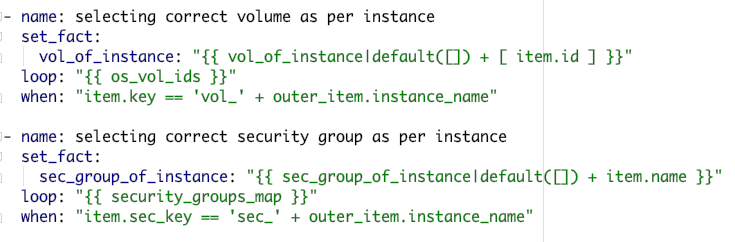
\includegraphics[width=13cm,keepaspectratio=true]{images/deployment/create_instance.png}
    \caption{Selecting security groups and volumes for respective instance}
    \label{fig:createinstance}
\end{figure}

\Challenge Docker APT repository configuration issue during installation

\TheSolution Due to the constraint of performing operations on the VMs using Ansible, this installation becomes pretty complicated. After reading several documentations, we were able to figure out the architecture requirement which was suitable for our linux machine, which turned out to be \texttt{amd64}.

\begin{figure}[H]
    \centering
    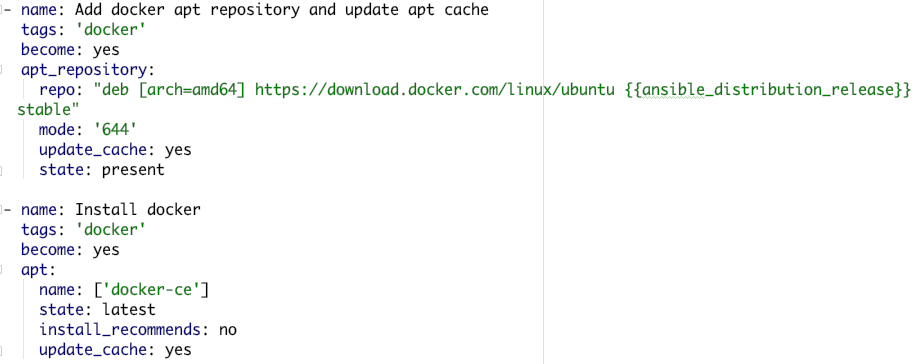
\includegraphics[width=13cm,keepaspectratio=true]{images/deployment/docker_repo_issue.png}
    \caption{Docker installation repository complication}
    \label{fig:dockerissue}
\end{figure}

\end{flattened}

\import{content/rohit/}{challenges.tex}